\section{问题四：固定联合任务的独立分组与资源配置}

\subsection{问题分析与固定前提}

问题四求解的是固定第三问联合任务后的资源分割问题，而不是运输—通信系统的再次联合优化。计算锁定问题三主方案中的货箱分配、多站航次、服务区顺序、机型、绝对起止时刻、三班中继的服务窗，以及4061个通信区间里的提供方。分组之后不重新拆箱、不更换机型、不平移时刻、不重新搜索中继，也不重新设计航线。各组仍使用问题三的绝对时钟，不是从各自的零时刻重新排程。若两组或三组独立执行，组与组之间不能共用运输机、运输电池、中继机或中继能源组件。共享取消以后，错峰使用过的实体要按组分别配置。因此，问题四的核心不是重新寻找运输路线，而是在固定联合时间表上求解不可拆任务分组及各组最低资源配置。

\subsection{服务区耦合与分组模型}

本节把不能拆开的服务区收成连通分量，并说明15个服务区为什么可以降成8个组件上的完整枚举。

\subsubsection{不可拆服务区图}

记$G=(V,E)$。$V$是15个服务区。若两个服务区出现在同一条问题三多站航次中，则连一条边：该航次只能属于一个执行组，两端服务区因此不能拆开。当前有边的航次是T003（S011—S015）、T004（S001—S013）、T010（S010—S009—S005）、T013（S013—S002）、T016（S006—S007）和T019（S007—S015）。T006与T021已在问题三中拆成单站，S009与S012之间没有边。连通分量就是不可拆组件，同一分量必须同组：
\begin{equation}
\begin{aligned}
C_1&=\{S001,S002,S013\},&
C_2&=\{S003\},&
C_3&=\{S004\},&
C_4&=\{S005,S009,S010\},\\
C_5&=\{S006,S007,S011,S015\},&
C_6&=\{S008\},&
C_7&=\{S012\},&
C_8&=\{S014\}.
\end{aligned}
\label{eq:components}
\end{equation}

\subsubsection{连通分量与组合空间降维}

直接划分15个服务区时，两个无标号非空组有$2^{14}-1=16383$种，三个组更多。多站航次把决策对象降为8个组件。$n$个互异对象分成$k$个无标号非空组的个数是第二类斯特林数，满足$S(n,1)=1$、$S(n,n)=1$以及
\begin{equation}
S(n,k)=k\,S(n-1,k)+S(n-1,k-1).
\label{eq:stirling}
\end{equation}
由此$S(8,2)=127$，$S(8,3)=966$。程序按分量下标把下一分量放入已有组或新开一组，每种无标号划分只生成一次；两组评价127次，三组966次，与这两个数相同，不是抽样碰巧得到的次数。图~\ref{fig:q4net}按这些航次画出八个分量。仅参与单站航次的服务区没有关联边，并单独形成一个连通分量。

\begin{figure}[H]\centering
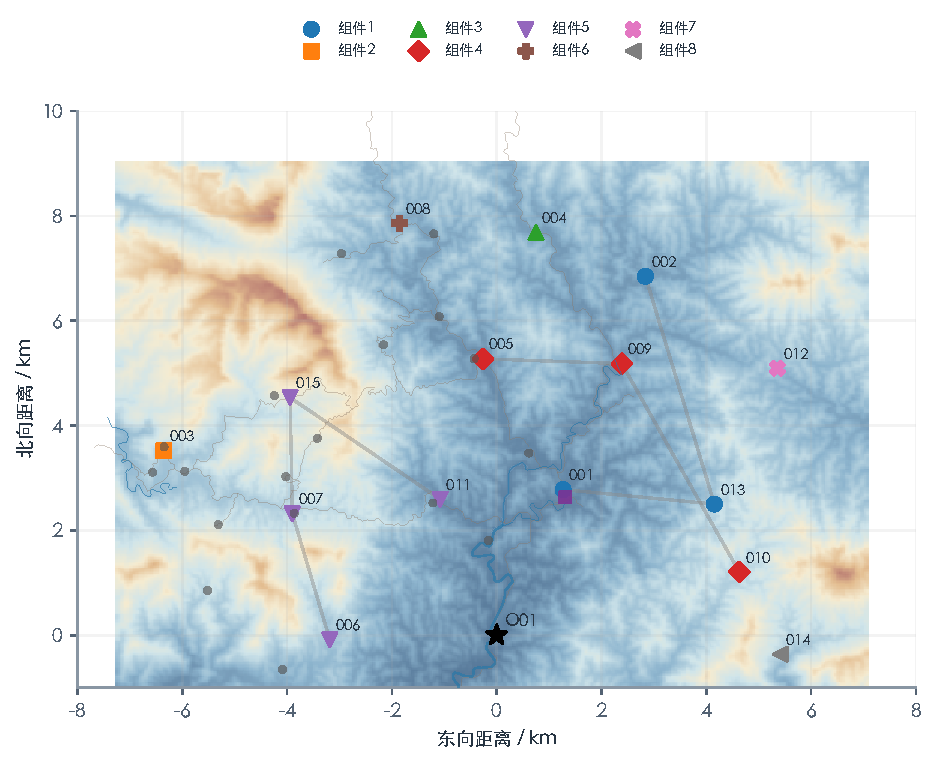
\includegraphics[width=.86\textwidth]{../figures/paper_full_20260926/q4_task_network.pdf}
\caption{问题三多站航次诱导的不可拆服务区组件}
\label{fig:q4net}
\end{figure}

\subsection{独立执行的资源配置模型}

在服务区分组确定后，需要计算每个独立小组必须自备的实体资源。本节在固定问题三绝对时间轴上建立资源峰值、跨组复制、库存缺口和工作量评价模型。

\subsubsection{固定时间轴下的资源峰值}

八类资源按固定顺序记为
\[
(N_A,N_B,N_C,N_{B_A},N_{B_B},N_{B_C},N_R,N_{B_R}),
\]
依次是A、B、C型运输机，三类电池，中继机和中继能源组件。附件库存为
\[
I=(4,2,2,6,4,4,2,6).
\]

组$h$、资源$r$的第$j$段占用记为$I_{j,r}^{(h)}$。固定时刻不能平移时，同一时刻重叠的任务不能共用一个实体，所以需求至少达到最大重叠数。区间图又可以用这么多个实体完成排布，因此最少实体数就等于最大并发：
\begin{equation}
N_r^{(h)}=\max_t\sum_j\mathbf{1}\{t\in I_{j,r}^{(h)}\}.
\label{eq:peak}
\end{equation}
它不等于航次条数。S012的T006b与T021b在1311~s至2049~s重叠，该组只有两条A型航次，仍需要2架A型机。

四类占用按代码分开计算，不混用。运输机取航次的$[t^{\rm start},t^{\rm end}]$。运输电池从同一起点延长到按返航SOC充满。中继机取$[t^{\rm start},t^{\rm end}]$再加题给的300~s周转；这是机体再次出动前的间隔，不是充电。中继能源组件从任务开始延长到组件充满，不含这300~s。机体周转和组件充电是两段不同的时间。

组间不能共享时，总需求是各组峰值之和，而不是全部任务放在同一时间轴上的一个峰值。记$n_{h,r}(t)$为组$h$在时刻$t$占用资源$r$的个数，则
\begin{equation}
\sum_h N_r^{(h)}
=\sum_h\max_t n_{h,r}(t)
\ge\max_t\sum_h n_{h,r}(t).
\label{eq:sumpeak}
\end{equation}
左边是独立配置，右边是未分组时的统一资源池。任务条数没有增加，左边仍可能更大，因为各组各自取最大值，错峰不再互相抵消。

\subsubsection{中继复制与能源组件占用}

中继的复制来自式~\eqref{eq:sumpeak}，而不是箱数变多。问题三里R02先执行RP02、再执行RP03，统一调度下可以是同一架机体，中继机峰值仍是2。两班若落到不同的组，各组都要自备一架，不能再串行复用。一个中继任务只要在证书里服务了某组的运输航次，独立执行后该组就要复制这一班，包括机体和一套能源组件。S014只使用RP02。把它单独成组后，必须自备1架中继机和1组能源组件，不能使用大组的R02。S003使用RP01、S012使用RP02时，再加上仍使用全部三班的大组所自备的2架，中继机数继续增加。具体入选划分见第\ref{sec:q4result}节。

能源组件还要计入充电拖尾。RP01的组件占用到8067~s。RP02占用到4764.061~s，RP03从4763.195~s开始，二者重叠约0.87~s，并与RP01同时在用，统一资源池的组件峰值已是3。重叠不到1~s，但绝对时刻不允许平移，这一秒仍然要另占一套组件。独立分组后再按组复制，组件数还会增加。

\subsubsection{资源缺口与工作量指标}

单项缺口、缺口总件数和配置总件数为
\begin{equation}
\delta_r=\max(0,N_r-I_r),\qquad
D=\sum_r\delta_r,\qquad
C=\sum_r N_r.
\label{eq:shortage}
\end{equation}
组$h$的工作时长是该组运输航次持续时间之和
\begin{equation}
W_h=\sum_{j\in h}D_j.
\label{eq:work}
\end{equation}
$D_j$是航次$j$在\texttt{route}中的\texttt{duration}：时钟从准备时间与起飞前装载时间起算，加上各航段的爬升、巡航和下降，其中包括返回调度中心的返航，并在每个服务区加上交接时间。返航后的电池充电和全部中继任务都不计入$D_j$。$K$个组的平均值$\mu_W$和总体标准差$\sigma_W$都除以$K$，不除以$K-1$，与计算程序的默认标准差一致。变异系数$\mathrm{CV}_W=\sigma_W/\mu_W$只比较上述运输航次时长，不比较箱数、能耗或人员负荷。

题目没有规定分组的优先顺序。本文采用字典序
\begin{equation}
\min_{\mathrm{lex}}(D,\,C,\,\mathrm{CV}_W).
\label{eq:lex}
\end{equation}
先减少超出库存的件数，缺口相同时减少独立配置的总规模，这两项相同时再比较工作时长是否接近。这是本文的建模选择，不是题目给定的唯一目标。

\subsection{两组与三组分组结果}
\label{sec:q4result}

127个二组划分和966个三组划分全部按式~\eqref{eq:lex}评价。本节先说明枚举比较的顺序，再分别解释入选的两组和三组，最后比较资源缺口与工作时长是否指向同一种划分。

\subsubsection{字典序目标与枚举方法}

每个划分都在固定时刻表上计算资源峰值，再得到缺口$D$、总配置$C$和工作时长变异系数$\mathrm{CV}_W$，然后按词典序比较。两组评价127次，三组966次，与$S(8,2)$和$S(8,3)$相同。入选方案是该组数下、这一限定空间内的字典序最优划分。

\subsubsection{两组方案}

字典序最小的两组方案把$C_8=\{S014\}$单独成组，其余七个分量为一组，箱数为77和3。S014只使用RP02，单独成组后必须自备1架中继机和1组能源组件，不能再使用大组的R02，中继机因此是$2+1=3$。它的1架B型机和1组B型电池也不能再计入未分组时的2架和4组，B型机和B型电池从2和4升到3和5。相对库存，缺的是1架B型运输机、1组B型电池和1架中继机，缺口总件数$D=3$，配置$C=31$。两组划分中，入选方案首先达到最小资源缺口$D=3$，并在缺口并列方案中继续按总配置量$C$和工作时长变异系数$\mathrm{CV}_W$进行词典序筛选，因此是127个二组划分中的字典序最优方案。

\subsubsection{三组方案}

字典序最小的三组方案把$C_2=\{S003\}$和$C_7=\{S012\}$分别成组，箱数为69、8和3。S003使用RP01、S012使用RP02，再加上大组的2架，中继机为4。为了不拆开多站航次，69箱留在一组，S003与S012成为两个较短的组，组间工作时长差异增大。缺口为2架A型机、1架C型机、2组A型电池和2架中继机，$D=7$，$C=36$；B型机和B型电池不再短缺。入选方案为966个三组划分中按$(D,C,\mathrm{CV}_W)$比较得到的字典序最优方案。工作时长的比较见图~\ref{fig:q4work}。

\subsubsection{资源与均衡性比较}

服务区与峰值见表~\ref{tab:q4group}，合计见表~\ref{tab:q4sum}。图~\ref{fig:partition}给出空间划分，图~\ref{fig:q4work}比较运输工作时长，图~\ref{fig:q4res}对照独立需求与库存。

\begin{table}[H]\centering\scriptsize
\caption{两组与三组方案的工作量及资源需求}\label{tab:q4group}
\resizebox{\textwidth}{!}{\begin{tabular}{llrrrr}\toprule
方案 & 服务区 & 箱数 & 工作时长/min & 资源向量 & 中继任务\\\midrule
两组甲 & 除S014外14个服务区 & 77 & 791.63 & $(4,2,2,6,4,4,2,3)$ & RP01--RP03\\
两组乙 & S014 & 3 & 31.16 & $(0,1,0,0,1,0,1,1)$ & RP02\\
三组甲 & 除S003、S012外13个服务区 & 69 & 675.08 & $(3,2,2,5,4,3,2,3)$ & RP01--RP03\\
三组乙 & S003 & 8 & 78.41 & $(1,0,1,1,0,1,1,1)$ & RP01\\
三组丙 & S012 & 3 & 69.30 & $(2,0,0,2,0,0,1,1)$ & RP02\\\bottomrule
\end{tabular}}\end{table}

\begin{table}[H]\centering\small
\caption{两组与三组方案的资源缺口、配置规模与工作量指标}\label{tab:q4sum}
\begin{tabular}{lrrrl}\toprule
方案 & $D$ & $C$ & $\mathrm{CV}_W$ & 资源缺口\\\midrule
库存 & --- & --- & --- & $(4,2,2,6,4,4,2,6)$\\
两组 & 3 & 31 & 0.9243 & $(0,1,0,0,1,0,1,0)$\\
三组 & 7 & 36 & 1.0335 & $(2,0,1,2,0,0,2,0)$\\\bottomrule
\end{tabular}\end{table}

\begin{figure}[H]\centering
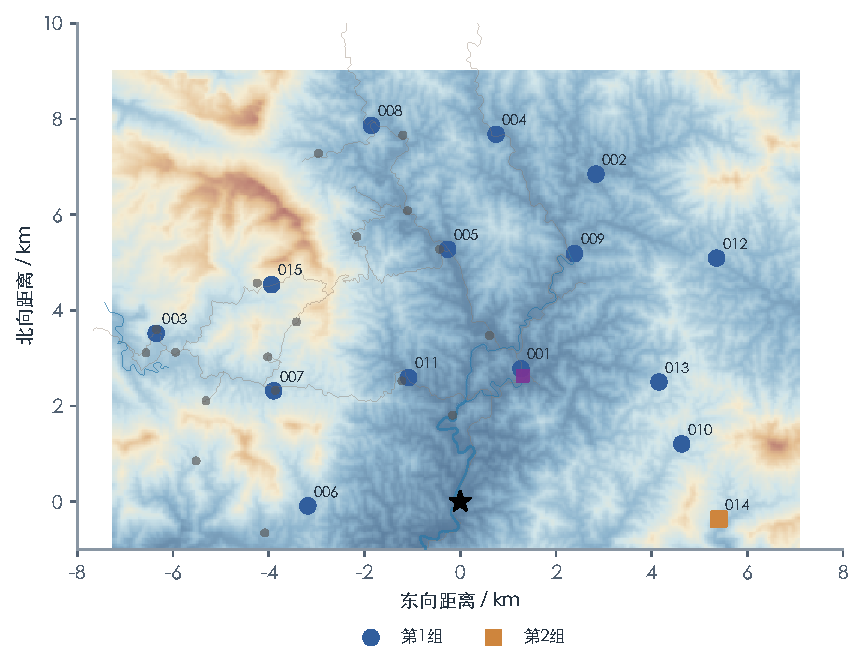
\includegraphics[width=.48\textwidth]{../figures/paper_full_20260926/q4_partition_2groups.pdf}
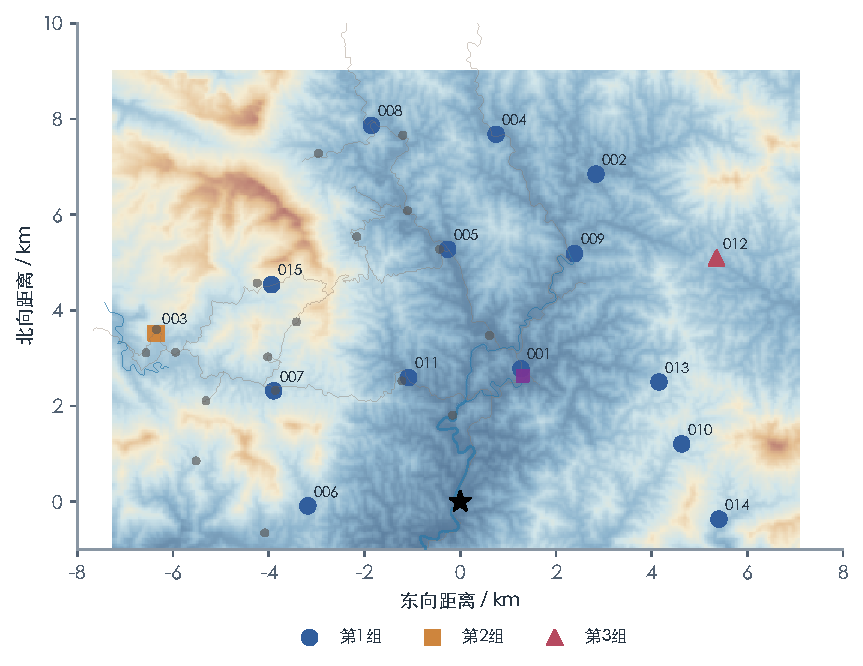
\includegraphics[width=.48\textwidth]{../figures/paper_full_20260926/q4_partition_3groups.pdf}
\caption{固定问题三任务下的两组与三组服务区划分}
\label{fig:partition}
\end{figure}

颜色仅表示独立执行组，不表示重新规划后的运输航线。图~\ref{fig:q4work}比较入选两组与三组方案的运输工作时长。三组方案中69箱任务集中在主组，另外两组仅承担8箱和3箱，因此$\mathrm{CV}_W$由0.9243升至1.0335，当前入选三组方案的工作时长并未更加均衡。按式~\eqref{eq:lex}，两组的缺口、配置件数和CV都更小。需求超过库存的部分构成式~\eqref{eq:shortage}定义的资源缺口。

\begin{figure}[H]\centering
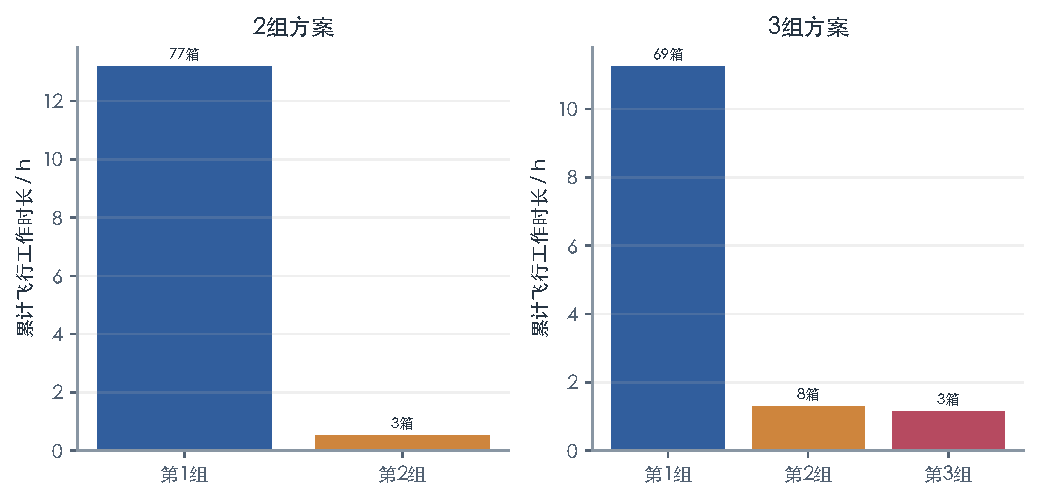
\includegraphics[width=.86\textwidth]{../figures/paper_full_20260926/q4_workload.pdf}
\caption{两组与三组方案的运输工作时长对比}
\label{fig:q4work}
\end{figure}


相对未分组时的统一峰值$(4,2,2,6,4,4,2,3)$，两组多配置的是$(0,1,0,0,1,0,1,1)$，能源组件仍闲置2组；三组多配置$(2,0,1,2,0,0,2,2)$，能源组件闲置1组。未分组时，问题三主方案的统一峰值没有超出库存。该峰值依赖统一资源池下的跨任务错峰复用，不能直接作为独立分组后的资源需求，也不能代替表~\ref{tab:q4sum}。三组再复制S003、S012的A型机、C型机和中继后，A型机从库存内的4架升到6架。闲置和缺口可以同时存在：能源组件库存有余，中继机体和部分运输资源却因式~\eqref{eq:sumpeak}被复制。资源配置最省的划分与工作时长最均衡的划分并不一致。

\begin{figure}[H]\centering
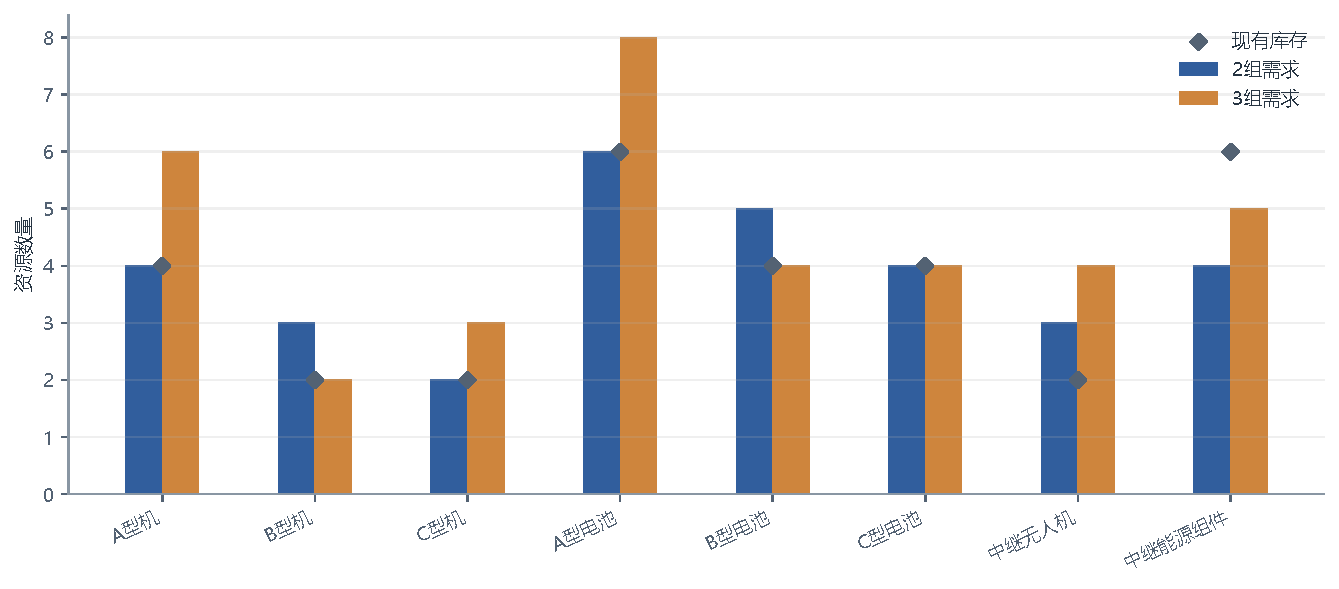
\includegraphics[width=.90\textwidth]{../figures/paper_full_20260926/q4_resource_demand.pdf}
\caption{独立执行资源需求与现有库存对比}
\label{fig:q4res}
\end{figure}

工作时长更接近的划分存在，但资源缺口更大。127个两组划分里，最小$\mathrm{CV}_W$约为$4.63\times10^{-4}$，对应43箱与37箱，缺口总件数13，配置43件。966个三组划分里，最小$\mathrm{CV}_W$约为0.0203，缺口总件数20，配置50件。式~\eqref{eq:lex}把缺口放在CV之前，这两个划分没有入选。

\subsection{分组结果与适用范围}

在问题三正式方案的箱组、服务顺序、机型、绝对任务时刻和通信关系保持不变，且资源需求按本文占用区间和式~\eqref{eq:peak}计算时，对全部127种二组划分和966种三组划分做了完整枚举。表~\ref{tab:q4group}分别是这两个限定空间内式~\eqref{eq:lex}的最优分组：两组$D=3$、$C=31$、$\mathrm{CV}_W=0.9243$，优于三组的$D=7$、$C=36$、$\mathrm{CV}_W=1.0335$。

按式~\eqref{eq:lex}的字典序评价，两组方案优于三组方案，因为独立组越多，原来在同一时间轴上错峰使用的机体和电池越不能跨组复用。三组把S003和S012再拆出去，复制了更多运输无人机和中继机，组间工作时长差异也更大。

本文没有重新设计运输航线、更换机型、平移任务时刻、改动中继部署，也没有让各组从零时刻重新排程。因此不能把当前缺口称为问题三与问题四的联合全局最优。$\mathrm{CV}_W$只比较运输航次持续时间。中继机体在返航后另加300~s周转，能源组件则延长到充满；改用别的占用定义，缺口会改变。
\addtocontents{toc}{\protect\setcounter{tocdepth}{3}}
